\documentclass[11pt, compress, aspectratio=1610, serif]{beamer}

\usetheme{pl}

\usepackage{booktabs}
\usepackage{minted}
\usepackage{listings}
\usepackage{color}
\usepackage{fancyvrb}
\newcommand{\VerbBar}{|}
\newcommand{\VERB}{\Verb[commandchars=\\\{\}]}
\DefineVerbatimEnvironment{Highlighting}{Verbatim}{commandchars=\\\{\}}
% Add ',fontsize=\small' for more characters per line
\newenvironment{Shaded}{}{}
\newcommand{\KeywordTok}[1]{\textcolor[rgb]{0.00,0.44,0.13}{\textbf{{#1}}}}
\newcommand{\DataTypeTok}[1]{\textcolor[rgb]{0.56,0.13,0.00}{{#1}}}
\newcommand{\DecValTok}[1]{\textcolor[rgb]{0.25,0.63,0.44}{{#1}}}
\newcommand{\BaseNTok}[1]{\textcolor[rgb]{0.25,0.63,0.44}{{#1}}}
\newcommand{\FloatTok}[1]{\textcolor[rgb]{0.25,0.63,0.44}{{#1}}}
\newcommand{\ConstantTok}[1]{\textcolor[rgb]{0.53,0.00,0.00}{{#1}}}
\newcommand{\CharTok}[1]{\textcolor[rgb]{0.25,0.44,0.63}{{#1}}}
\newcommand{\SpecialCharTok}[1]{\textcolor[rgb]{0.25,0.44,0.63}{{#1}}}
\newcommand{\StringTok}[1]{\textcolor[rgb]{0.25,0.44,0.63}{{#1}}}
\newcommand{\VerbatimStringTok}[1]{\textcolor[rgb]{0.25,0.44,0.63}{{#1}}}
\newcommand{\SpecialStringTok}[1]{\textcolor[rgb]{0.73,0.40,0.53}{{#1}}}
\newcommand{\ImportTok}[1]{{#1}}
\newcommand{\CommentTok}[1]{\textcolor[rgb]{0.38,0.63,0.69}{\textit{{#1}}}}
\newcommand{\DocumentationTok}[1]{\textcolor[rgb]{0.73,0.13,0.13}{\textit{{#1}}}}
\newcommand{\AnnotationTok}[1]{\textcolor[rgb]{0.38,0.63,0.69}{\textbf{\textit{{#1}}}}}
\newcommand{\CommentVarTok}[1]{\textcolor[rgb]{0.38,0.63,0.69}{\textbf{\textit{{#1}}}}}
\newcommand{\OtherTok}[1]{\textcolor[rgb]{0.00,0.44,0.13}{{#1}}}
\newcommand{\FunctionTok}[1]{\textcolor[rgb]{0.02,0.16,0.49}{{#1}}}
\newcommand{\VariableTok}[1]{\textcolor[rgb]{0.10,0.09,0.49}{{#1}}}
\newcommand{\ControlFlowTok}[1]{\textcolor[rgb]{0.00,0.44,0.13}{\textbf{{#1}}}}
\newcommand{\OperatorTok}[1]{\textcolor[rgb]{0.40,0.40,0.40}{{#1}}}
\newcommand{\BuiltInTok}[1]{{#1}}
\newcommand{\ExtensionTok}[1]{{#1}}
\newcommand{\PreprocessorTok}[1]{\textcolor[rgb]{0.74,0.48,0.00}{{#1}}}
\newcommand{\AttributeTok}[1]{\textcolor[rgb]{0.49,0.56,0.16}{{#1}}}
\newcommand{\RegionMarkerTok}[1]{{#1}}
\newcommand{\InformationTok}[1]{\textcolor[rgb]{0.38,0.63,0.69}{\textbf{\textit{{#1}}}}}
\newcommand{\WarningTok}[1]{\textcolor[rgb]{0.38,0.63,0.69}{\textbf{\textit{{#1}}}}}
\newcommand{\AlertTok}[1]{\textcolor[rgb]{1.00,0.00,0.00}{\textbf{{#1}}}}
\newcommand{\ErrorTok}[1]{\textcolor[rgb]{1.00,0.00,0.00}{\textbf{{#1}}}}
\newcommand{\NormalTok}[1]{{#1}}

\makeatletter
\def\maxwidth{\ifdim\Gin@nat@width>\linewidth\linewidth\else\Gin@nat@width\fi}
\makeatother

\usepgfplotslibrary{dateplot}

\newcommand{\begincols}{\begin{columns}}
\newcommand{\stopcols}{\end{columns}}

\title{Title}
\subtitle{Subtitle}
\date{\today}
\author{Timothée Poisot}
\institute{Université de Montréal}

\begin{document}

\maketitle

\begin{frame}{A slide}

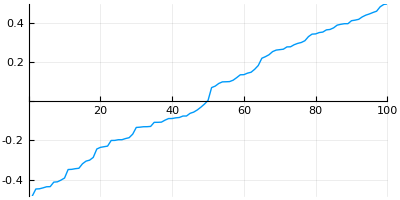
\includegraphics[width=\textwidth]{figures/density.png}

\end{frame}

\begin{frame}{A frame with maths}

\[
\frac{1}{N}\frac{\text{d}}{\text{d}t}N = N\left(r-\alpha N\right)
\]

What about symbols, \(B_x \forall x \in \sum_i k_i \leq 2\), and
integration \(x = \int_i^\infty y_i\)?

\end{frame}

\section{Plots}\label{plots}

\begin{frame}[fragile]{Setting things up}

\begin{Shaded}
\begin{Highlighting}[]
\NormalTok{using Plots}
\NormalTok{pyplot()}
\end{Highlighting}
\end{Shaded}

\begin{verbatim}
Plots.PyPlotBackend()
\end{verbatim}

\end{frame}

\begin{frame}[fragile]{Columns}

\begincols
\column{0.48\textwidth}

\begin{Shaded}
\begin{Highlighting}[]
\NormalTok{p1 = plot(}
  \CommentTok{# These are the data}
  \NormalTok{sort(rand(}\FloatTok{40}\NormalTok{)),}
  \CommentTok{# This is the plot size}
  \NormalTok{size  = (}\FloatTok{250}\NormalTok{, }\FloatTok{200}\NormalTok{),}
  \CommentTok{# We don't want borders}
  \NormalTok{frame = :grid,}
  \CommentTok{# We don't want a legend}
  \NormalTok{leg   = false}
  \NormalTok{);}
\NormalTok{savefig(p1, }\StringTok{"figures/scatter.pdf"}\NormalTok{);}
\end{Highlighting}
\end{Shaded}

\hfill\column{0.48\textwidth}

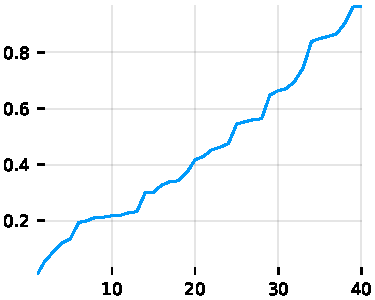
\includegraphics[width=\columnwidth]{figures/scatter.pdf}

\stopcols

\end{frame}

\begin{frame}{Output}

Pellentesque habitant morbi tristique senectus et netus et malesuada
fames ac turpis egestas. Morbi sollicitudin nisi vitae lorem interdum,
eget elementum quam elementum. Curabitur quis leo eu metus consequat
ultricies. Curabitur sit amet convallis risus. Cras vel arcu id risus
efficitur commodo et eget velit. Curabitur consequat eleifend magna, ut
ultricies lorem scelerisque eu. Mauris faucibus neque sit amet est
elementum, suscipit placerat est interdum. Phasellus sed convallis est.
Nunc fermentum convallis odio eget gravida. Duis venenatis dictum
tempor.

\end{frame}

\section{Some code}\label{some-code}

\begin{frame}{Default plotting}

Some text maybe?

\end{frame}

\frame[plain]{Thank you}

\end{document}
